\section{Semaine 08 (18/11-22/11) }


\e{Notions abordées :}
\begin{itemize}
	\item Oscillateur harmonique (cf semaine précédente).
	\item Oscillateur amorti.
\end{itemize}

\subsection{Questions de cours}

\begin{enumerate}
	\item Établir l'équation d'un circuit $RLC$ série.
	\item Donner l'équation de l'oscillateur amorti et ses solutions dans le cas général.
	\item Résoudre l'équation de l'oscillateur harmonique avec les conditions initiales $u(0)=3E$ et $\dot{u}(0)=4 \omega E$. Quelle est la phase à l'origine ?
\end{enumerate}

\subsection{Exercice 1 : Exemple de régime critique}

\begin{minipage}[c]{\linewidth/2}
	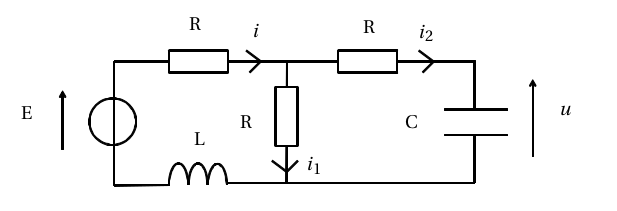
\includegraphics[width=\textwidth]{./Images/mpsi_s08_ex01.png}
\end{minipage}%
\begin{minipage}[c]{\linewidth/2}
	Initialement le condensateur est déchargé et aucun courant ne traverse la bobine.
\end{minipage}

\begin{enumerate}
	\item Déterminer l'équation différentielle vérifiée par $u(t)$.
	\item Quelle est la relation entre $R$, $L$ et $C$ pour vérifier la condition de régime critique ? On suppose cette condition vérifiée dans la suite.
	\item Quelles sont les conditions initiales ? Déterminer également $u(\infty)$ et $i(\infty)$.
	\item Déterminer $u(t)$.
\end{enumerate}

\e{Réponses :}
\begin{enumerate}
	\item $u'' + 1/2(3R/L + 1/RC)u' + u/LC = E/2LC$
	\item $L = R^2 C$
	\item $u=0$, $u'=0$.
	\item $u(t) = E/2 - E/2(1+t/RC)e^{-t/RC}$
\end{enumerate}

\subsection{Exercice 2 : Étude d'un circuit à deux bobines}

\begin{minipage}[c]{\linewidth/2}
	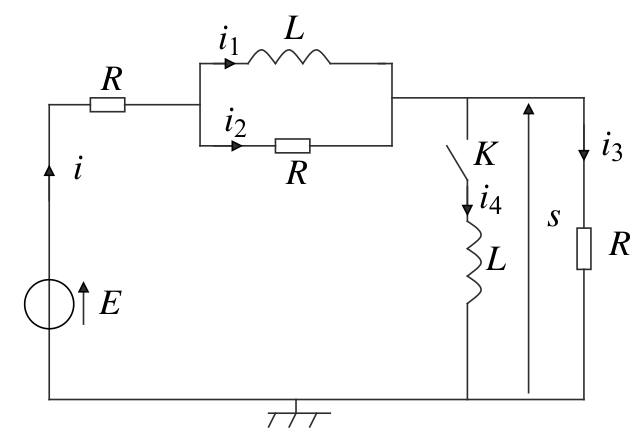
\includegraphics[width=\textwidth]{./Images/mpsi_s08_ex02.png}
\end{minipage}%
\begin{minipage}[c]{\linewidth/2}
	À $t=0$, on ferme $K$
\end{minipage}

\begin{enumerate}
	\item Établir l'équation différentielle vérifiée par $s(t)$.
	\item Déterminer les conditions initiales pour $i$, $i_1$, $i_2$, $i_3$ et $i_4$. Déterminer également leurs valeurs pour $t\rightarrow+\infty$.
	\item Déterminer $s(t)$. 
\end{enumerate}

\e{Réponses :}
\begin{enumerate}
	\item $3s'' + 4R/L s' + (R/L)^2 s = 0$
	\item En $t=0^+$, $i_1=E/2R$, $i_3=E/2R$, $i=E/R$, $i_2=0$, $i_4=0$.
	\item $s(t) = \frac{E}{4} \left( \exp -\frac{R}{L}t +  \exp -\frac{R}{3L}t \right)$
\end{enumerate}


\subsection{Exercice 3 : Réponse à un échelon de tension d'un dipôle $RLC$ parallèle}

\begin{minipage}[c]{\linewidth/2}
	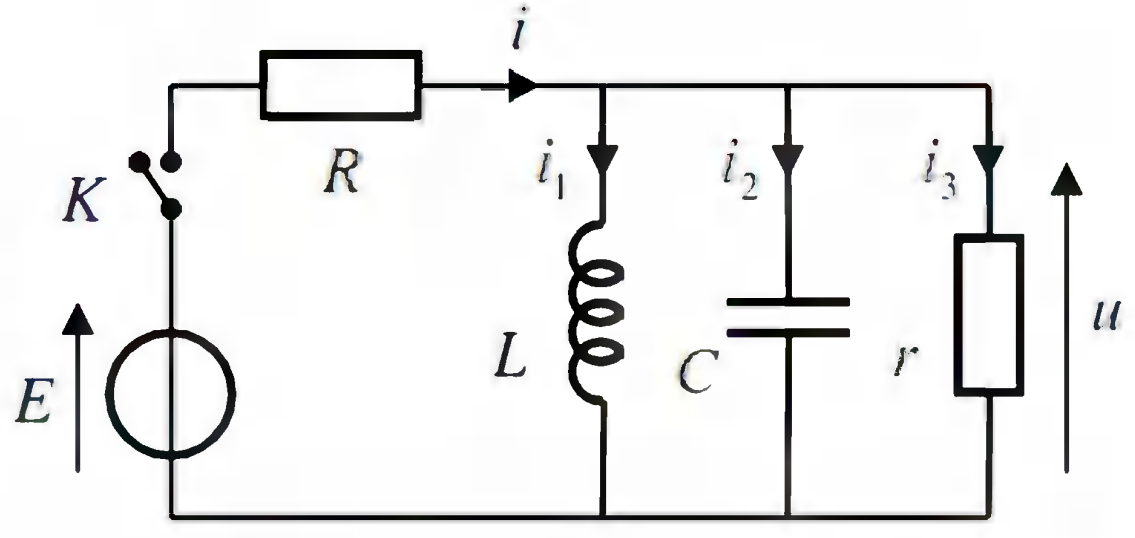
\includegraphics[width=\textwidth]{./Images/mpsi_s08_ex03.png}
\end{minipage}%
\begin{minipage}[c]{\linewidth/2}
	Pour $t<0$, le condensateur est déchargé et la bobine idéale n'est parcourue par aucun courant. À $t=0$, on ferme $K$
\end{minipage}

\begin{enumerate}
	\item Établir l'équation différentielle vérifiée par $i_3$. La mettre sous forme canonique.
	\item Déterminer les conditions initiales. Déterminer également la valeur de $i_3$ pour $t\rightarrow+\infty$.
	\item Donner la relation entre $R$, $r$, $L$ et $C$ pour que le régime soit de type pseudopériodique et exprimer $i_3(t)$ dans ce cas.
\end{enumerate}

\e{Réponses :}
\begin{enumerate}
	\item $\omega_0 = \frac{1}{\sqrt{LC}}$, $\frac{\omega_0}{Q} = \frac{R + r}{RrC}$.
	\item En $t=0^+$, $u=0$, $i_1=0$, $i_3=0$, $i=E/R$, $i_2=E/R$. En $t\rightarrow+\infty$, $u=0$, $i=i_1=E/R$, $i_2=i_3=0$
	\item $\frac{2rR}{R+r} > \sqrt{\frac{L}{C}}$
\end{enumerate}

